\begin{frame}[label = kelley2013Datasets]
	\frametitle{ Multi-model scores}
	\framesubtitle{Model scores}
	
	% Smileys
	\foreach \x in {1, 2, 3, 4, 5, 6, 7} {
		\only<\x> {
			\includegraphics[width=10cm]{images/modelScores/pp\x.png}
	}}
	%Fire and veg
\end{frame}

\begin{frame}[label = kelley2013Datasets]
	\frametitle{JULES-INFERNO v obs}
	\framesubtitle{Model scores}
	
	\begin{textblock*}{8cm}(11cm ,1.3cm)
		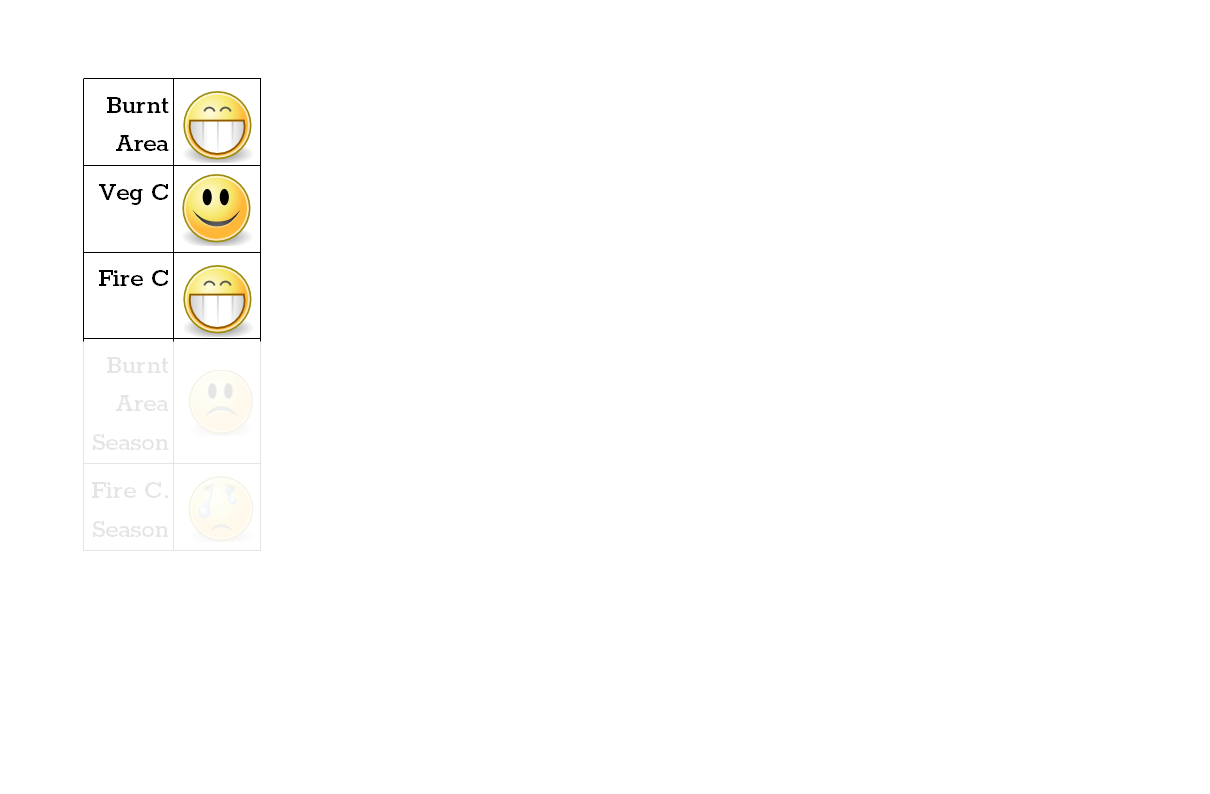
\includegraphics[width=7.5cm]{images/Smileys/BAvegCFireC.png}
	\end{textblock*}
	
	\only<2-> {
		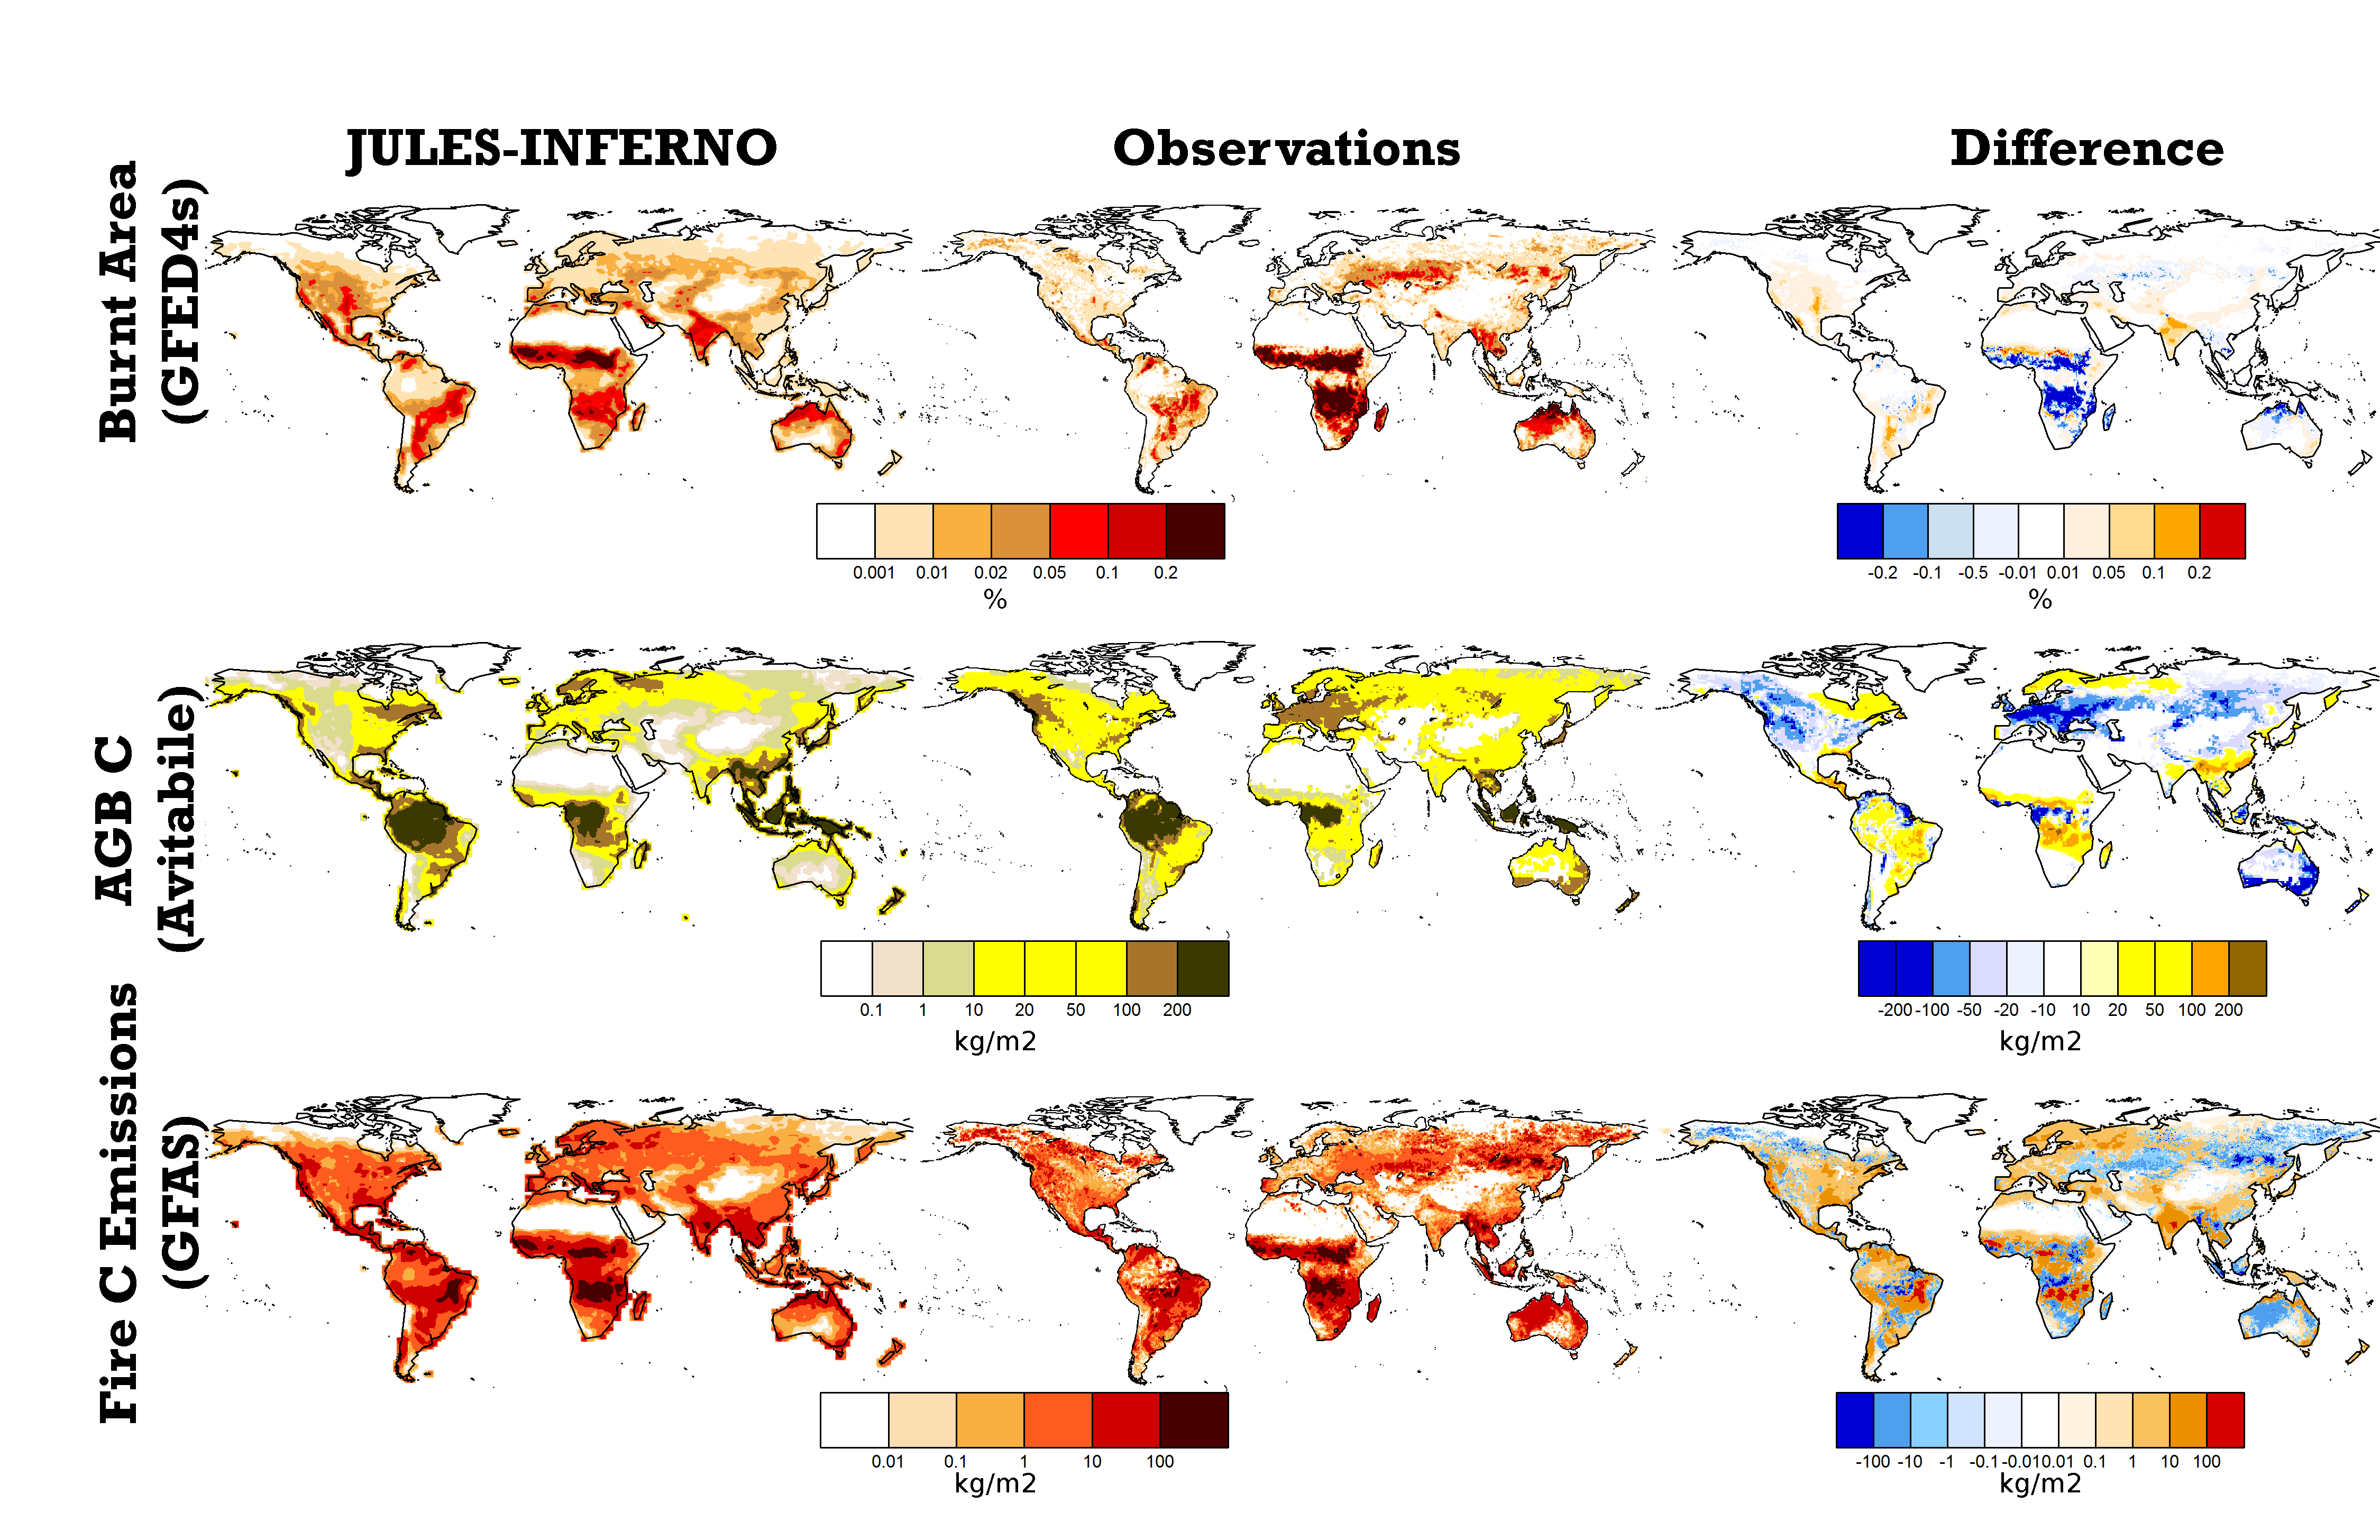
\includegraphics[width=10cm]{images/julesPerformance/FireMapsSpatial.png}
	}
\end{frame}

\begin{frame}[label = kelley2013Datasets]
	\frametitle{Multi-model scores}
	\framesubtitle{Model scores}
	
	\begin{textblock*}{8cm}(11cm ,1.3cm)
		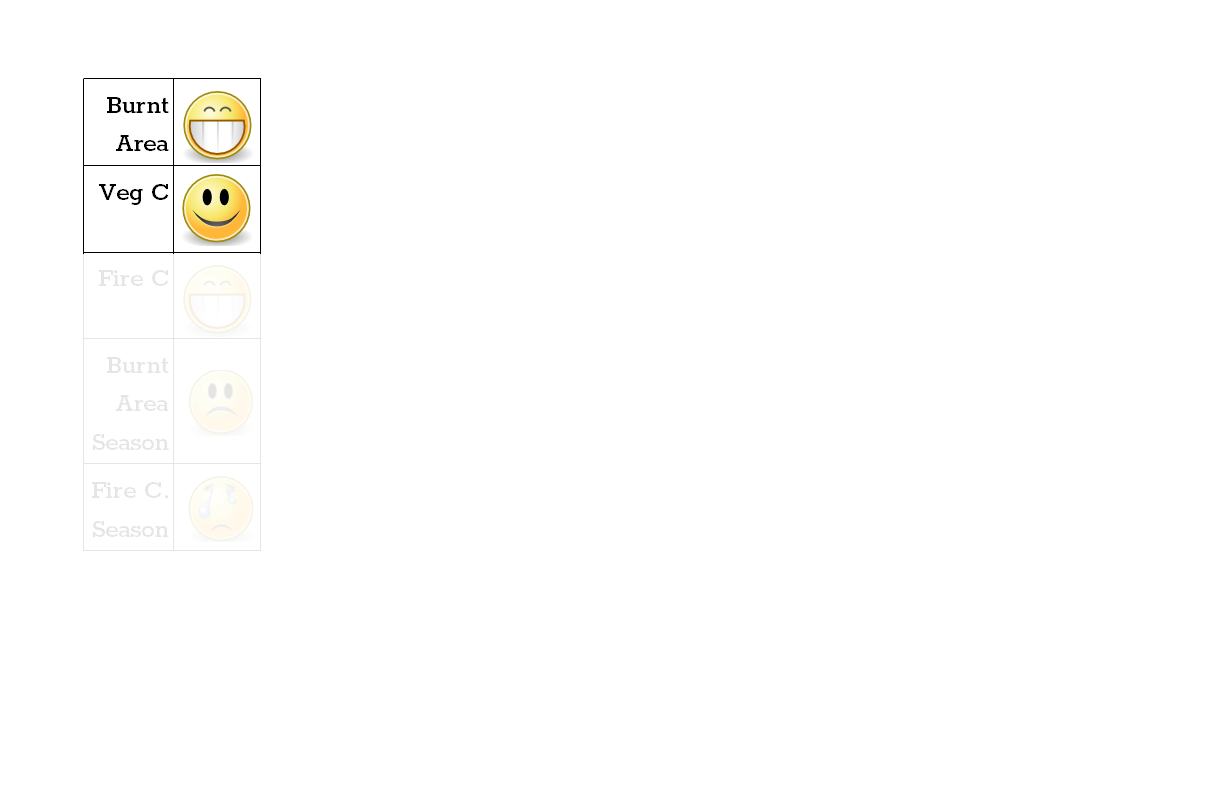
\includegraphics[width=7.5cm]{images/Smileys/BAvegC.png}
	\end{textblock*}
	
	\foreach \x in {1, 2} {
		\only<\x> {
			\includegraphics[width=10cm]{images/fireVsVegScores/pp\x.png}
	}}

\end{frame}



\begin{frame}[label = kelley2013Datasets]
	\frametitle{JULES-INFERNO v obs}
	\framesubtitle{Model scores}
	
	\begin{textblock*}{8cm}(11cm ,1.3cm)
		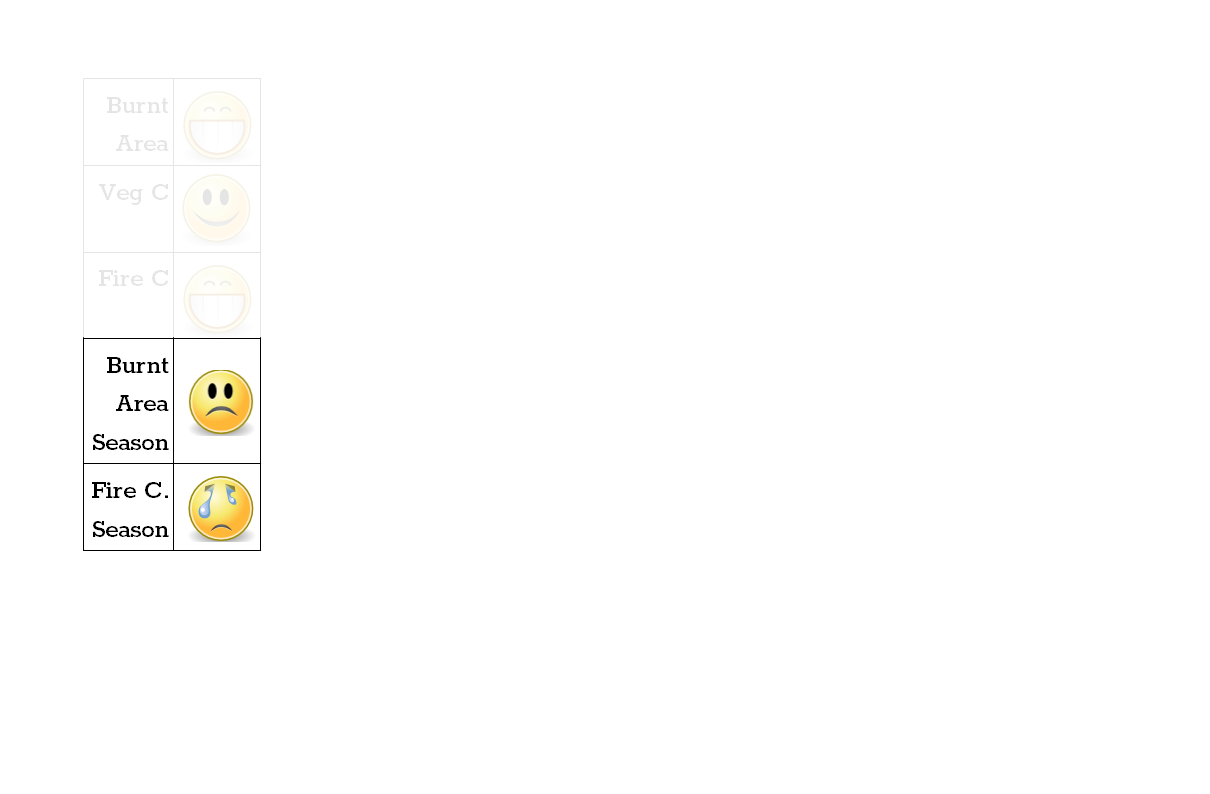
\includegraphics[width=7.5cm]{images/Smileys/BAFireCseason.png}
	\end{textblock*}
	
	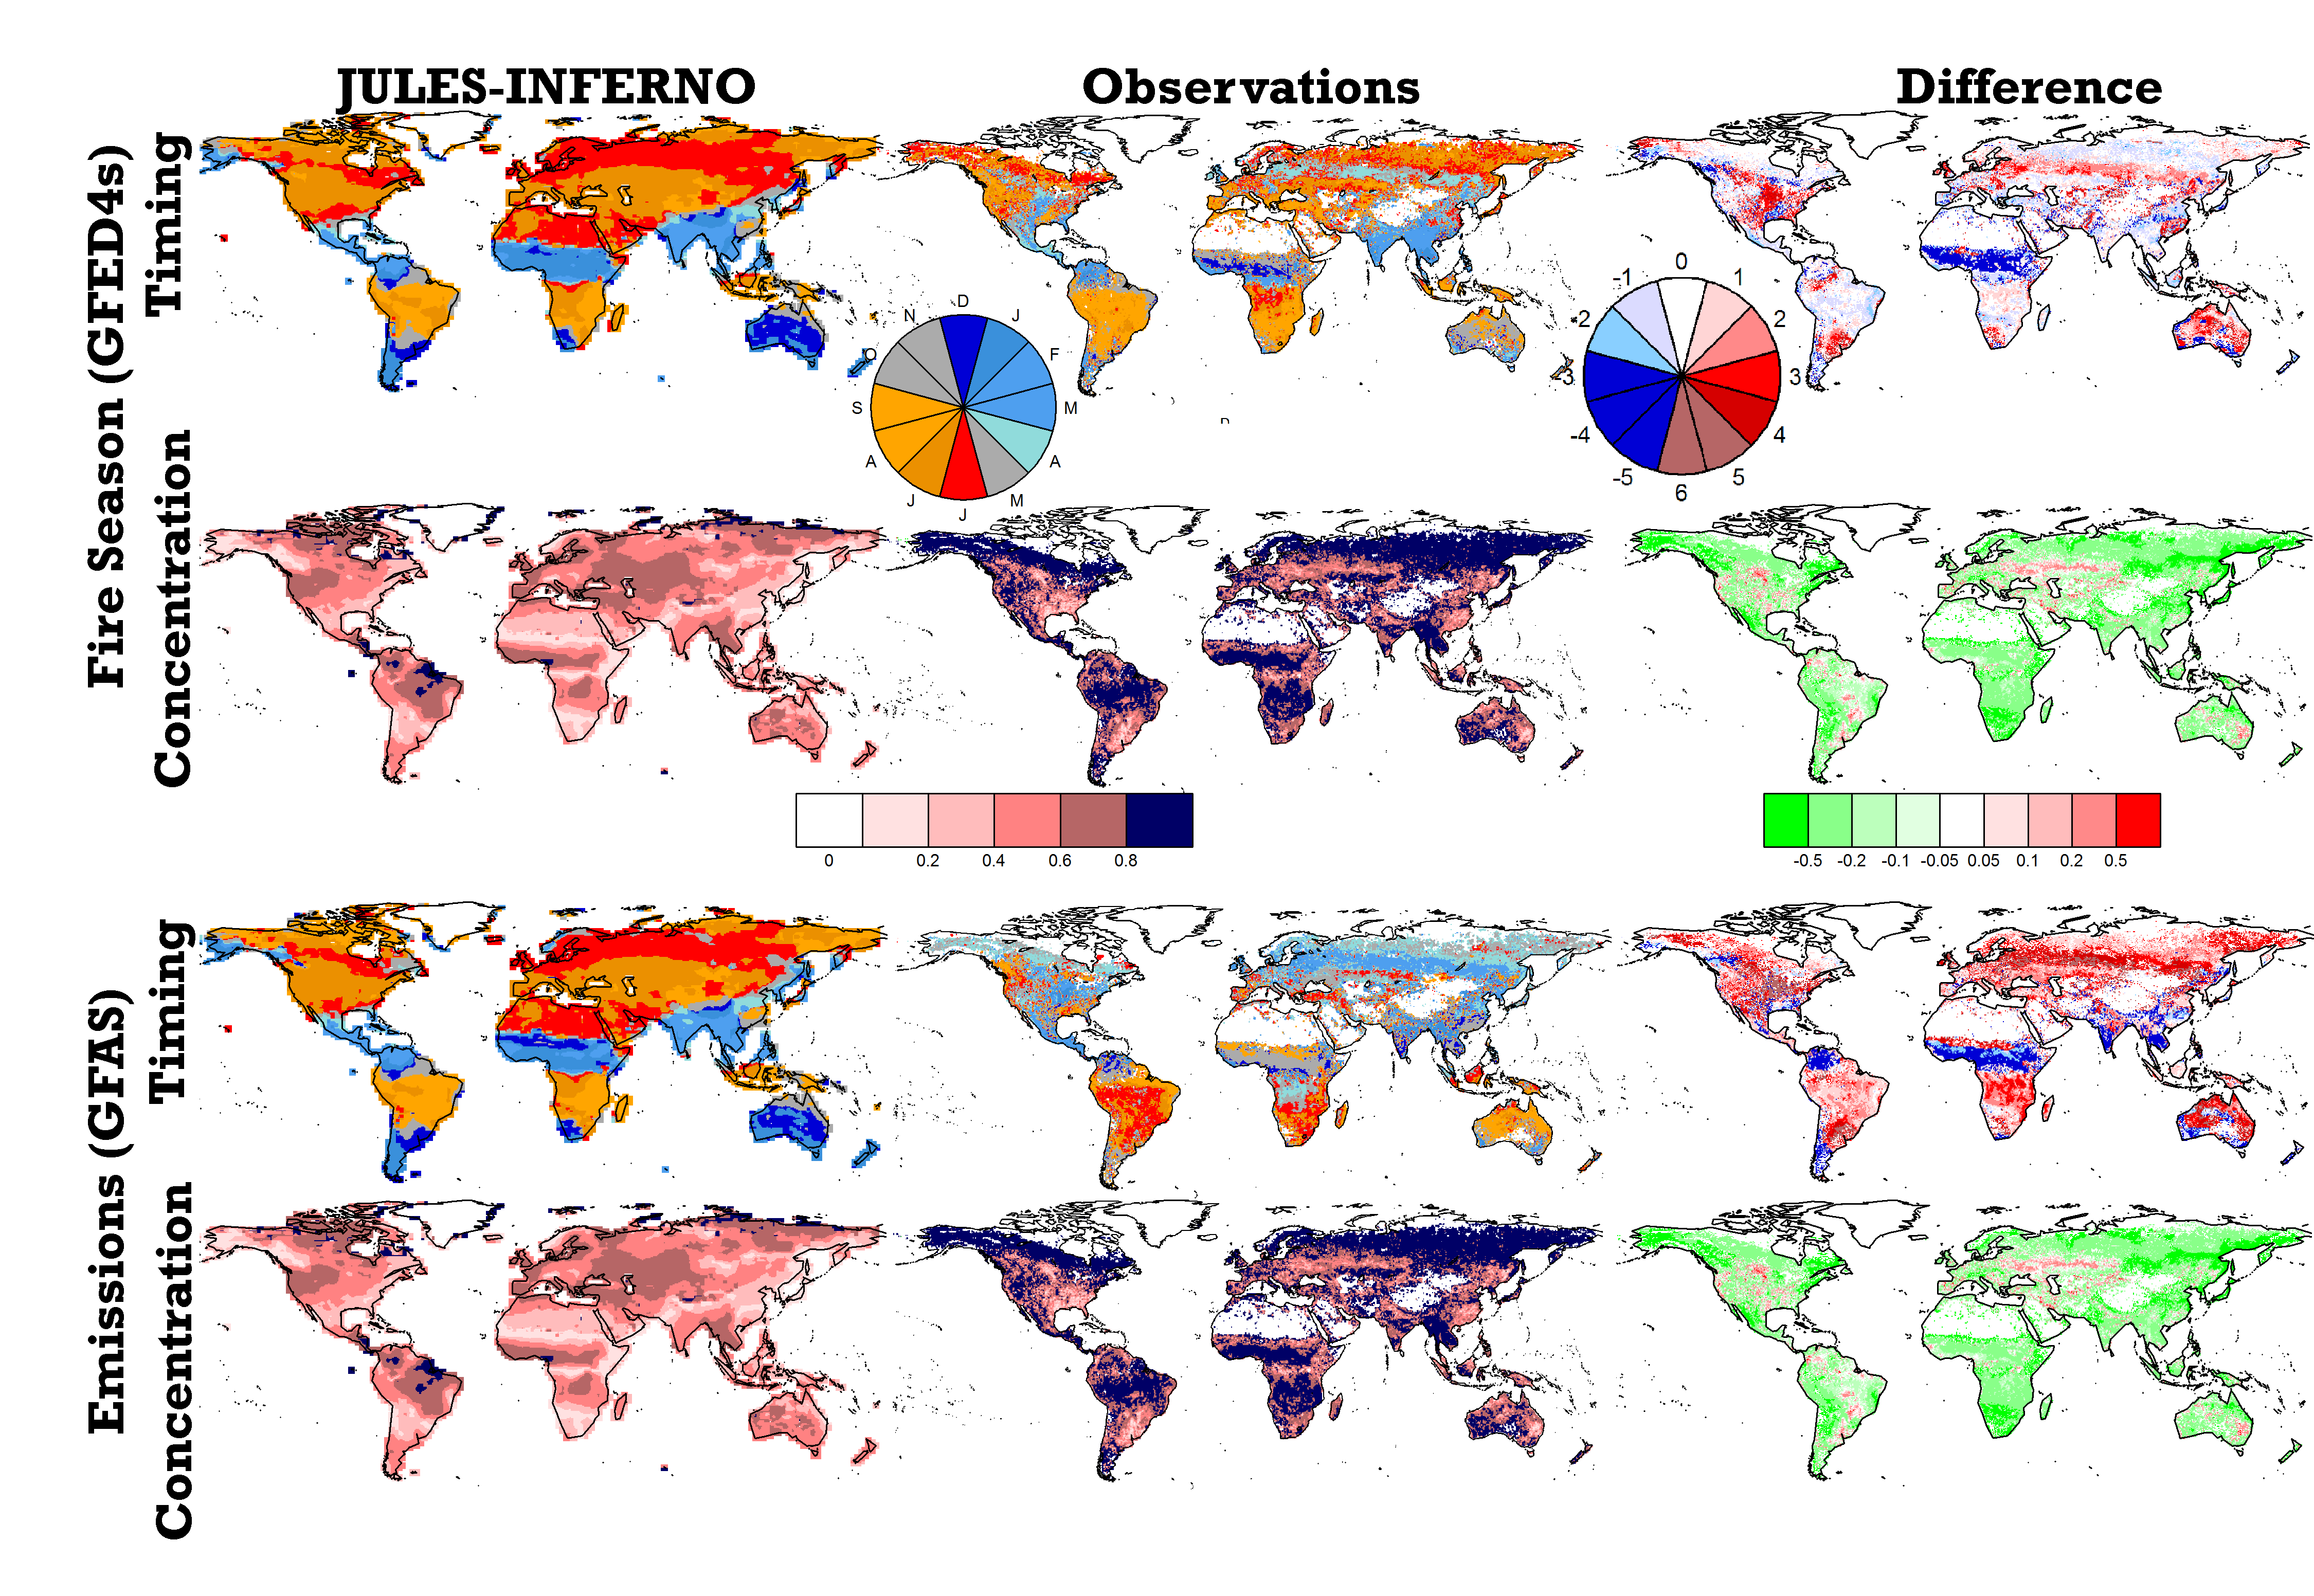
\includegraphics[width=10cm]{images/julesPerformance/FireMapsSeason.png}
	
\end{frame}

%\begin{frame}[label = kelley2013Datasets]
%	\frametitle{Model type scores}
%	\framesubtitle{Model scores}
%	
%	% Model types scores
%\end{frame}
